\documentclass[letterpaper,11pt,oneside,reqno]{article}

%%%%%%%%%%%%%%%%%%%%%%%%%%%%%%%%%%%%%%%%%%%%%%%%%%%%%%%%%%%%

\usepackage[pdftex,backref=page,colorlinks=true,linkcolor=blue,citecolor=red]{hyperref}
\usepackage[alphabetic,nobysame]{amsrefs}

%%%%%%%%%%%%%%%%%%%%%%%%%%%%%%%%%%%%%%%%%%%%%%%%%%%%%%%%%%%%
%main packages
\usepackage{amsmath,amssymb,amsthm,amsfonts,mathtools}
\usepackage{graphicx,color}
\usepackage{upgreek}
\usepackage[mathscr]{euscript}

%equations
\allowdisplaybreaks
\numberwithin{equation}{section}

%tikz
\usepackage{tikz}
\usetikzlibrary{shapes,arrows,positioning,decorations.markings}

%conveniences
\usepackage{array}
\usepackage{adjustbox}
\usepackage{cleveref}
\usepackage{enumerate}
\usepackage{datetime}

%paper geometry
\usepackage[DIV=12]{typearea}

%%%%%%%%%%%%%%%%%%%%%%%%%%%%%%%%%%%%%%%%%%%%%%%%%%%%%%%%%%%%
%draft-specific
\synctex=1
% \usepackage{refcheck,comment}

%%%%%%%%%%%%%%%%%%%%%%%%%%%%%%%%%%%%%%%%%%%%%%%%%%%%%%%%%%%%
%this paper specific
\newcommand{\ssp}{\hspace{1pt}}

%%%%%%%%%%%%%%%%%%%%%%%%%%%%%%%%%%%%%%%%%%%%%%%%%%%%%%%%%%%%
\newtheorem{proposition}{Proposition}[section]
\newtheorem{lemma}[proposition]{Lemma}
\newtheorem{corollary}[proposition]{Corollary}
\newtheorem{theorem}[proposition]{Theorem}
%%%%%%%%%%%%%%%%%%%%%%%%%%%%%%%%%%%%%%%%%%%%%%%%%%%%%%%%%%%%
\theoremstyle{definition}
\newtheorem{definition}[proposition]{Definition}
\newtheorem{remark}[proposition]{Remark}
\newtheorem{example}[proposition]{Example}
%%%%%%%%%%%%%%%%%%%%%%%%%%%%%%%%%%%%%%%%%%%%%%%%%%%%%%%%%%%%

\begin{document}
\title{Lectures on Random Matrices
(Spring 2025)
\\Lecture 1: Moments of random variables and random
matrices}


\date{Monday, January 13, 2025\footnote{\href{https://lpetrov.cc/rmt25/}{\texttt{Course webpage}}
$\bullet$ \href{https://lpetrov.cc/rmt25/rmt25-notes/rmt2025-l01.tex}{\texttt{TeX Source}}
$\bullet$
Updated at \currenttime, \today}}



\author{Leonid Petrov}


\maketitle


\section{Why study random matrices?}

\paragraph{On the history.}
Random matrix theory (RMT) is a fascinating field that
studies
properties of matrices with randomly generated entries,
focusing (at least initially)
on the statistical behavior of their eigenvalues.
This theory finds its roots in the domain of nuclear
physics through the pioneering work of Wigner, Dyson, and
others \cite{wigner1955characteristic},
\cite{dyson1962brownian},
\cite{Dyson1962_III}, who utilized it to analyze the energy levels of complex quantum systems.
Other, earlier roots include statistics \cite{dixon1905generalization}
and classical Lie groups \cite{Hurwitz1897}.
Today, RMT has evolved to span a wide array of disciplines,
from pure mathematics, including areas such as integrable
systems and representation theory, to practical applications
in fields like data science and engineering.

\paragraph{Classical groups and Lie theory.}
Random matrices are deeply connected to \emph{classical Lie groups}, particularly the orthogonal, unitary, and symplectic groups. This connection emerges primarily due to the invariance properties of these groups, such as those derived from the Haar measure.
Random matrices significantly impact representation theory, linking to integrals over matrix groups through character expansions. The symmetry classes of random matrix ensembles, like the Gaussian Orthogonal (GOE), Unitary (GUE), and Symplectic (GSE), correspond to respective symmetry groups.

\paragraph{Toolbox.}
RMT utilizes a broad range of tools ranging across all of mathematics, including probability theory, combinatorics, analysis (classical and modern), algebra, representation theory, and number theory.
The theory of random matrices is a rich source of problems and techniques for all of mathematics.

\paragraph{Applications.}
Random matrix theory finds applications across a diverse set
of fields. In nuclear physics, random matrix ensembles serve
as models for complex quantum Hamiltonians, thereby
explaining the statistics of energy levels. In number
theory, connections have been drawn between random matrices
and the Riemann zeta function, particularly concerning the
distribution of zeros on the critical line. Wireless
communications benefit from random matrix theory through the
analysis of eigenvalue distributions, which helps in
understanding channel capacity in multi-antenna (MIMO) systems. In the burgeoning field of
machine learning, random weight matrices and their spectra
are key to analyzing neural networks and their
generalization capabilities. High-dimensional statistics
and econometrics
also draw on random matrix tools for tasks such as principal
component analysis and covariance estimation in large
datasets. Additionally, combinatorial random processes
exhibit connections to random permutations, random graphs,
and partition theory, all through the lens of matrix
integrals.

\section{Recall Central Limit Theorem}

\subsection{Central Limit Theorem and examples}

We begin by establishing the necessary groundwork for understanding and proving
the Central Limit Theorem. The theorem's power lies in its remarkable universality:
it applies to a wide variety of probability distributions under mild conditions.

\begin{definition}
A sequence of random variables $\{X_i\}_{i=1}^{\infty}$ is said to be
\emph{independent and identically distributed (iid)}
if:

\begin{itemize}
    \item Each $X_i$ has the same probability distribution as every other $X_j$, for all $i, j$.
    \item The variables are mutually independent, meaning that for any finite subset $\{X_1, X_2, \dots, X_n\}$, the joint distribution factors as the product of the individual distributions:
    \[
			\operatorname{\mathbb{P}}(X_1 \leq x_1, X_2 \leq x_2, \dots, X_n \leq x_n)
			=
			\operatorname{\mathbb{P}}(X_1 \leq x_1)
			\operatorname{\mathbb{P}}(X_2 \leq x_2) \cdots \operatorname{\mathbb{P}}(X_n \leq x_n).
    \]
\end{itemize}
\end{definition}

\begin{theorem}[Classical Central Limit Theorem]
	Let $\{X_i\}_{i=1}^{\infty}$ be a sequence of iid random variables with finite mean $\mu = \operatorname{\mathbb{E}}[X_i]$ and finite
	variance $\sigma^2 = \operatorname{\mathrm{Var}}(X_i)$.
	Define the normalized sum
\[
Z_n = \frac{1}{\sqrt{n}} \sum_{i=1}^n \left(X_i - \mu\right).
\]
Then, as $n \to \infty$, the distribution of $Z_n$ converges in distribution to a normal random variable with mean $0$ and variance $\sigma^2$, i.e.,
\[
Z_n \xrightarrow{d} \mathcal{N}(0, \sigma^2).
\]
\end{theorem}
Convergence in distribution means
\begin{equation}
	\label{eq:conv-in-dist}
	\lim_{n \to \infty} \operatorname{\mathbb{P}}(Z_n \leq x) = \operatorname{\mathbb{P}}(Z \leq x)
		= \int_{-\infty}^x \frac{1}{\sqrt{2\pi \sigma^2}}\ssp e^{-\frac{t^2}{2\sigma^2}} \, dt
	\qquad
	\text{for all } x \in \mathbb{R},
\end{equation}
where $Z \sim \mathcal{N}(0, \sigma^2)$ is the Gaussian random variable.

\begin{remark}
	For a general random variable instead of
	$Z\sim \mathcal{N}(0, \sigma^2)$, the convergence in distribution
	\eqref{eq:conv-in-dist} holds only for $x$ at which the cumulative distribution function of $Z$ is continuous.
	Since the normal distribution is absolutely continuous (has density), the convergence holds for all $x$.
\end{remark}
\begin{figure}[htpb]
	\centering
	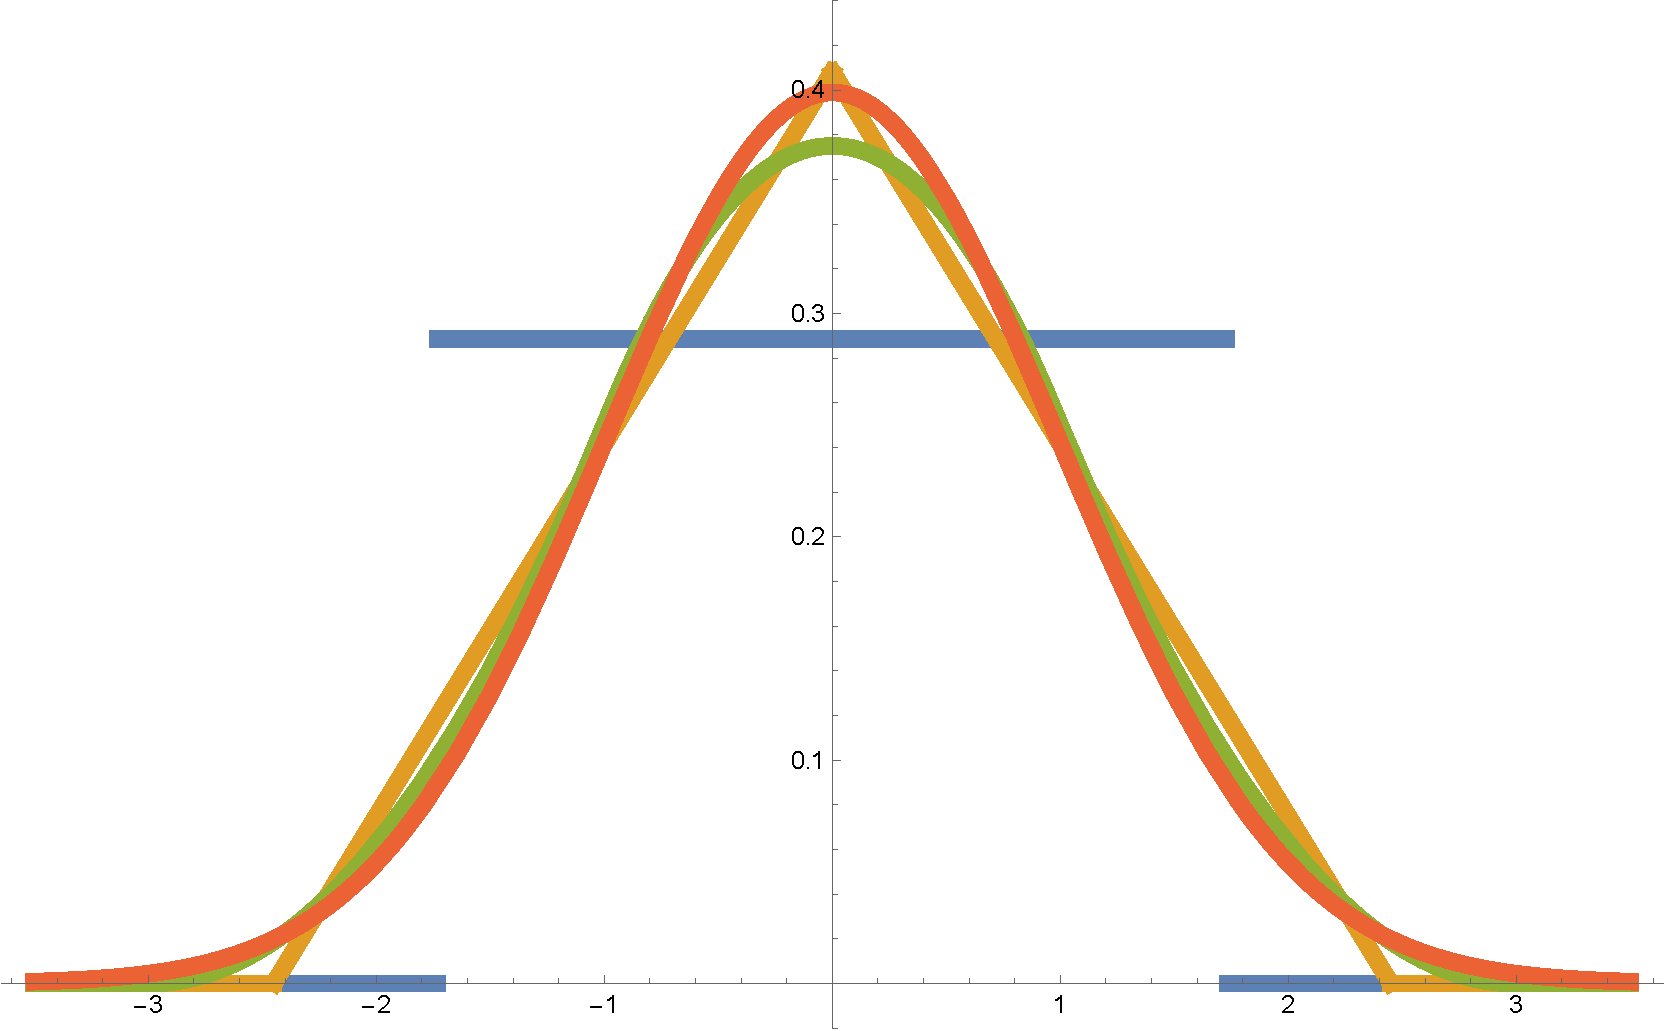
\includegraphics[width=0.5\textwidth]{./pictures/uniform_pdfs.pdf}
	\caption{Densities of $U_1$, $U_1+U_2$, $U_1+U_2+U_3$ (where $U_i$ are iid uniform on $[0,1]$),
		and $\mathcal{N}(0,1)$,
		normalized to have the same mean and variance.}
	\label{fig:uniform_pdfs}
\end{figure}

\begin{example}
Let $\{X_i\}_{i=1}^{\infty}$ be a sequence of iid Bernoulli random variables with parameter $p$, meaning that each $X_i$ takes the value $1$ with probability $p$ and $0$ with probability $1 - p$. The mean and variance of each $X_i$ are given by:
\[
	\mu = \operatorname{\mathbb{E}}[X_i] = p, \quad \sigma^2 = \operatorname{\mathrm{Var}}(X_i) = p(1 - p).
\]
We also have the distribution of $X_1+\cdots+X_n$:
\begin{equation*}
	\operatorname{\mathbb{P}}\left( X_1+ \cdots + X_n = k \right) = \binom{n}{k} p^k (1-p)^{n-k},
	\qquad k = 0, 1, \ldots, n.
\end{equation*}

\colorbox{yellow}{\parbox{.7\textwidth}{local CLT via Stirling}}

\end{example}


\subsection{Moments of the normal distribution}

\begin{proposition}
The moments of a random variable $Z \sim \mathcal{N}(0, \sigma^2)$ are given by:
\begin{equation}
	\label{eq:normal-moments}
	\operatorname{\mathbb{E}}[Z^k] = \begin{cases}
		0, & \text{if } k \text{ is odd}, \\
		\sigma^k (k-1)!! = \sigma^k \cdot (k-1)(k-3) \cdots 1, & \text{if } k \text{ is even}.
	\end{cases}
\end{equation}
\end{proposition}
\begin{proof}
	We just compute the integrals. Assume $k$ is even (for odd,
	the integral is zero by symmetry). Also assume $\sigma = 1$ for simplicity.
	Then
\begin{equation*}
	\operatorname{\mathbb{E}}[Z^k]
	=
	\frac{1}{\sqrt{2\pi}}
	\int_{-\infty}^{\infty}  z^k e^{-z^2/2} \, dz.
\end{equation*}
Applying integration by parts (putting $ze^{-z^2/2}$ under $d$), we get
\begin{equation*}
	\operatorname{\mathbb{E}}[Z^k] = \frac{1}{\sqrt{2\pi}} \left[-z^{k-1}e^{-z^2/2}\right]_{-\infty}^{\infty} + \frac{k-1}{\sqrt{2\pi}} \int_{-\infty}^{\infty} z^{k-2} e^{-z^2/2} \, dz.
\end{equation*}
The first term vanishes at infinity (you can verify this using L'Hôpital's rule), leaving us with:
\begin{equation*}
	\operatorname{\mathbb{E}}[Z^k] = (k-1)\operatorname{\mathbb{E}}[Z^{k-2}].
\end{equation*}
This gives us a recursive formula, and completes the proof.
\end{proof}




\subsection{Moments of sums of iid random variables}








































\bibliographystyle{alpha}
\bibliography{bib}


\medskip

\textsc{L. Petrov, University of Virginia, Department of Mathematics, 141 Cabell Drive, Kerchof Hall, P.O. Box 400137, Charlottesville, VA 22904, USA}

E-mail: \texttt{lenia.petrov@gmail.com}


\end{document}
